% 1956 年全国卷第 7 题：等边三角形外接圆上的点 P 与 AP、BC 交点 M。
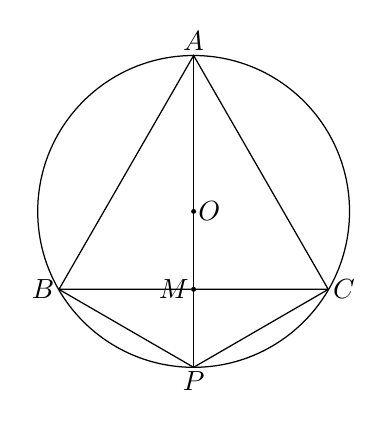
\begin{tikzpicture}[scale=0.9, line width=0.45pt,
  every node/.style={inner sep=1.5pt}]
  \coordinate (O) at (0,0);
  \coordinate (A) at (0,2.2);
  \coordinate (B) at (-1.9,-1.1);
  \coordinate (C) at (1.9,-1.1);
  \coordinate (P) at (0,-2.2);
  \coordinate (M) at (0,-1.1);
  \draw (O) circle (2.2);
  \draw (A)--(B)--(C)--cycle;
  \draw (A)--(P);
  \draw (B)--(P)--(C);
  \draw (B)--(C);
  \fill (O) circle (0.035) (M) circle (0.035);
  \node[anchor=south] at (A) {$A$};
  \node[anchor=east] at (B) {$B$};
  \node[anchor=west] at (C) {$C$};
  \node[anchor=north] at (P) {$P$};
  \node[anchor=west] at (O) {$O$};
  \node[anchor=east] at (M) {$M$};
\end{tikzpicture}
